
\documentclass{beamer}
\usecolortheme{dove}
\setbeamertemplate{navigation symbols}{}
\usepackage{amsmath,amssymb,amsfonts,amsthm, multicol, subfigure, color}
\usepackage{bm}
\usepackage{graphicx}
\usepackage{tabularx}
\usepackage{booktabs}
\usepackage{hyperref}
\usepackage{pdfpages}
\usepackage{xcolor}
\definecolor{seagreen}{RGB}{46, 139, 87}
\def\independenT#1#2{\mathrel{\rlap{$#1#2$}\mkern2mu{#1#2}}}
\newcommand\indep{\protect\mathpalette{\protect\independenT}{\perp}}
\def\log{\text{log}}
\newcommand\logit{\text{logit}}
\newcommand\iid{\stackrel{\text{iid}}{\sim}}
\newcommand\E{\text{E}}
\newcommand\V{\text{V}}
\renewcommand\P{\text{P}}
\newcommand{\Cov}{\text{Cov}}
\newcommand{\Cor}{\text{Cor}}
\newcommand\doop{\texttt{do}}
\usepackage{stackrel}
\usepackage{tikz}
\usetikzlibrary{arrows,shapes.arrows,positioning,shapes,patterns,calc}
\newcommand\slideref[1]{\vskip .1cm \tiny \textcolor{gray}{{#1}}}
\newcommand\red[1]{\color{red}#1}
\newcommand\blue[1]{\color{blue}#1}
\newcommand\gray[1]{\color{gray}#1}
\newcommand\seagreen[1]{\color{seagreen}#1}
\newcommand\purple[1]{\color{purple}#1}
\newcommand\orange[1]{\color{orange}#1}
\newcommand\black[1]{\color{black}#1}
\newcommand\white[1]{\color{white}#1}
\newcommand\teal[1]{\color{teal}#1}
\newcommand\magenta[1]{\color{magenta}#1}
\newcommand\Fuchsia[1]{\color{Fuchsia}#1}
\newcommand\BlueGreen[1]{\color{BlueGreen}#1}
\newcommand\bblue[1]{\textcolor{blue}{\textbf{#1}}}
\newcommand\bred[1]{\textcolor{red}{\textbf{#1}}}
\newcommand\bgray[1]{\textcolor{gray}{\textbf{#1}}}
\newcommand\bgreen[1]{\textcolor{seagreen}{\textbf{#1}}}
\newcommand\bref[2]{\href{#1}{\color{blue}{#2}}}
\colorlet{lightgray}{gray!40}
\pgfdeclarelayer{bg}    % declare background layer for tikz
\pgfsetlayers{bg,main} % order layers for tikz
\newcommand\mycite[1]{\begin{scriptsize}\textcolor{darkgray}{(#1)}\end{scriptsize}}
\newcommand{\tcframe}{\frame{
%\small{
\only<1|handout:0>{\tableofcontents}
\only<2|handout:1>{\tableofcontents[currentsubsection]}}
%}
}

\usepackage[round]{natbib}
\bibliographystyle{humannat-mod}
\setbeamertemplate{enumerate items}[default]
\usepackage{mathtools}

% Need to add examples

\newcommand{\goalsframe}{\begin{frame}{Learning goals for today}
At the end of class, you will be able to:
\begin{enumerate}
\item Define natural direct and indirect effects
\item Decompose total effects into these components
\item Understand how intermediate confounding complicates natural direct effects
\item Estimate natural direct and indirect effects
\end{enumerate} \vskip .2in
\end{frame}}

\title{18. Mediation:\\Natural Direct and Indirect Effects}
\author{Ian Lundberg\\Cornell Info 6751: Causal Inference in Observational Settings\\Fall 2022}
\date{25 Oct 2022}

\begin{document}

\maketitle

\goalsframe

\begin{frame}[t]{Recall from before: Controlled direct effects} \vskip .1in
\begin{center}
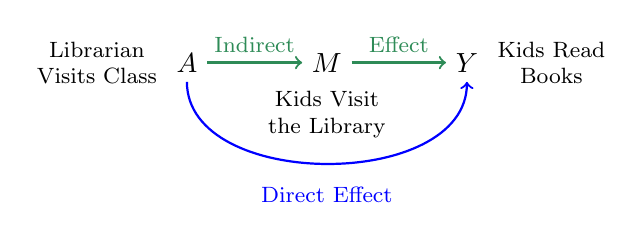
\begin{tikzpicture}[x = 1in, y = .7in, every node/.style = {anchor=center}]
%\node at (-1,-1.6) {};
\node (y) at (1.4,0) {$Y$};
\node[anchor = west, font = \footnotesize, align = center] at (y.east) {Kids Read\\Books};
\node (A) at (0,0) {$A$};
\node[anchor = east, font = \footnotesize, align = center] at (A.west) {Librarian\\Visits Class};
\node (M) at (.7,0) {$M$};
\node[anchor = north, font = \footnotesize, align = center] at (M.south) {Kids Visit\\the Library};
\draw[->, thick, seagreen] (A) -- node[midway, above, font = \footnotesize, seagreen] {Indirect} (M);
\draw[->, thick, seagreen] (M) -- node[midway, above, font = \footnotesize, seagreen] {Effect} (y);
\draw[->, thick, blue] (A) to[bend right = 90] node[midway, below, font = \footnotesize, outer sep = 5pt] {Direct Effect} (y);
\end{tikzpicture} \vskip .2in \pause
\end{center}
Direct effect: Close the library
$$\E\left(Y^{10} - Y^{00}\right)$$ \vskip .1in \pause
Direct effect: Make everyone visit the library
$$\E\left(Y^{11} - Y^{01}\right)$$

\end{frame}

\begin{frame}[t]{Today: Natural direct effects} \vskip .1in
\begin{center}
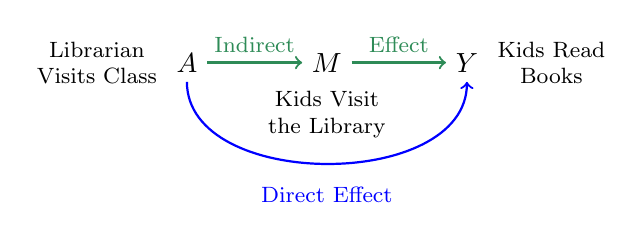
\begin{tikzpicture}[x = 1in, y = .7in, every node/.style = {anchor=center}]
%\node at (-1,-1.6) {};
\node (y) at (1.4,0) {$Y$};
\node[anchor = west, font = \footnotesize, align = center] at (y.east) {Kids Read\\Books};
\node (A) at (0,0) {$A$};
\node[anchor = east, font = \footnotesize, align = center] at (A.west) {Librarian\\Visits Class};
\node (M) at (.7,0) {$M$};
\node[anchor = north, font = \footnotesize, align = center] at (M.south) {Kids Visit\\the Library};
\draw[->, thick, seagreen] (A) -- node[midway, above, font = \footnotesize, seagreen] {Indirect} (M);
\draw[->, thick, seagreen] (M) -- node[midway, above, font = \footnotesize, seagreen] {Effect} (y);
\draw[->, thick, blue] (A) to[bend right = 90] node[midway, below, font = \footnotesize, outer sep = 5pt] {Direct Effect} (y);
\end{tikzpicture} \vskip .2in \pause
\end{center}
Let $M^a$ be the potential mediator value under treatment $A = a$ \vskip .1in \pause
Direct effect (0): Effect of the librarian visiting in a world where kids visit the library as if the librarian didn't visit the class
$$\E\left(Y^{1M^0} - Y^{0M^0}\right)$$ \vskip .1in \pause
Direct effect (1): Effect of the librarian visiting in a world where kids visit the library as if the librarian visited the class
$$\E\left(Y^{1M^1} - Y^{0M^1}\right)$$

\end{frame}

\begin{frame}{Natural direct and indirect effects: Decomposition}

The total effect can be decomposed into two components \pause
$$\begin{aligned}
&\E\bigg(Y^1 - Y^0\bigg) &\text{Total effect} \\ \pause
&= \E\bigg(Y^{1M^1} - Y^{0M^0}\bigg) &\text{since }Y^{a}=Y^{aM^a} \\ \pause
&= \E\bigg(Y^{1M^1} \underbrace{- Y^{1M^0} + Y^{1M^0}}_\text{Add 0} - Y^{0M^0}\bigg) \\ \pause
&= \underbrace{\E\bigg(Y^{1M^1} - Y^{1M^0}\bigg)}_{\substack{\text{\bblue{Indirect Effect}}\\\text{(effect through $M$)}}} + \underbrace{\E\bigg(Y^{1M^0} - Y^{0M^0}\bigg)}_{\substack{\text{\bblue{Direct Effect}}\\\text{(effect not through $M$)}}}
\end{aligned}$$

\end{frame}

\begin{frame}{Indirect effect: Interpretation}
\begin{center}
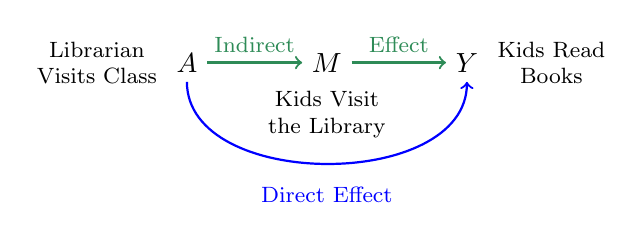
\begin{tikzpicture}[x = 1in, y = .7in, every node/.style = {anchor=center}]
\node (y) at (1.4,0) {$Y$};
\node[anchor = west, font = \footnotesize, align = center] at (y.east) {Kids Read\\Books};
\node (A) at (0,0) {$A$};
\node[anchor = east, font = \footnotesize, align = center] at (A.west) {Librarian\\Visits Class};
\node (M) at (.7,0) {$M$};
\node[anchor = north, font = \footnotesize, align = center] at (M.south) {Kids Visit\\the Library};
\draw[->, thick, seagreen] (A) -- node[midway, above, font = \footnotesize, seagreen] {Indirect} (M);
\draw[->, thick, seagreen] (M) -- node[midway, above, font = \footnotesize, seagreen] {Effect} (y);
\draw[->, thick, blue] (A) to[bend right = 90] node[midway, below, font = \footnotesize, outer sep = 5pt] {Direct Effect} (y);
\end{tikzpicture} \vskip .2in \pause
\end{center}
\onslide<3->{Indirect effect (1): Effect of visiting the library as much as you would if the librarian did vs did not visit,\\in a world where the librarian visits}
$$\tau(1) = \E(Y^{1M^1} - Y^{1M^0})$$
\onslide<4->{Indirect effect (0): Effect of visiting the library as much as you would if the librarian did vs did not visit,\\in a world where the librarian does not visit}
$$\tau(0) = \E(Y^{0M^1} - Y^{0M^0})$$
\end{frame}

\begin{frame}{Controlled and natural direct effects:\\Context of controlled experiments}
\begin{tikzpicture}[x = \textwidth, y = .8\textheight]
\node[anchor = north west] at (0,1) {Controlled direct effect};
\node[anchor = north west] at (.5,1) {Natural direct effect};
\node[anchor = north west] at (0,.9) {$\frac{1}{n}\sum_{i=1}^n \bigg(Y_i^{11} - Y_i^{01}\bigg)$};
\node[anchor = north west] at (.5,.9) {$\frac{1}{n}\sum_{i=1}^n \bigg(Y_i^{1M_i^1} - Y_i^{0M_i^1}\bigg)$}; \pause
\node[anchor = north west, font = \footnotesize, align = left] at (0,.7) {$Y_i^{11}$ can be observed\\in an experiment};
\node[anchor = north west, font = \footnotesize, align = left] at (0,.58) {--- Assign $A = 1$ and $M =1$}; \pause
\node[anchor = north west, font = \footnotesize, align = left] at (0,.5) {$Y_i^{01}$ can be observed\\in an experiment};
\node[anchor = north west, font = \footnotesize, align = left] at (0,.38) {--- Assign $A = 0$ and $M =1$}; \pause
\node[anchor = north west, font = \footnotesize, align = left] at (.5,.7) {$Y_i^{1M_i^1}$ can be observed\\in an experiment};
\node[anchor = north west, font = \footnotesize, align = left] at (.5,.58) {--- Assign $A = 1$}; \pause
\node[anchor = north west, font = \footnotesize, align = left] at (.5,.5) {$Y_i^{0M_i^1}$ \bblue{cannot} be observed\\in an experiment};
\node[anchor = north west, font = \footnotesize, align = left] at (.5,.38) {--- Because $M_i^1$ is unknown!};
\end{tikzpicture}
\end{frame}

\begin{frame}{The unobservable potential outcome:\\An experimental solution} \pause
Crossover design\footnote{Imai, K., Tingley, D., \& Yamamoto, T. (2013). \bref{https://doi.org/10.1111/j.1467-985X.2012.01032.x}{Experimental designs for identifying causal mechanisms.} Journal of the Royal Statistical Society: Series A (Statistics in Society), 176(1), 5-51.}
\begin{itemize} \pause
\item In period 1, assign $A = a$. See outcome $M = M^a$ \pause
\item In period 2, assign $A = a'$. Assign $M = M^a$. See $Y^{a'M^a}$ \pause
\end{itemize} \vskip .2in
Works an assumption of no carry-over:\\current treatment is all that affects current outcome
\end{frame}

\begin{frame}[t]{Intermediate confounding: A threat to natural effects} \vskip .08in
\begin{center}
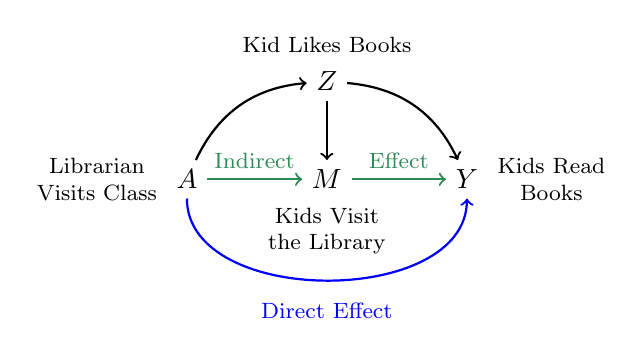
\begin{tikzpicture}[x = 1in, y = .7in, every node/.style = {anchor=center}]
\node (y) at (1.4,0) {$Y$};
\node[anchor = west, font = \footnotesize, align = center] at (y.east) {Kids Read\\Books};
\node (A) at (0,0) {$A$};
\node[anchor = east, font = \footnotesize, align = center] at (A.west) {Librarian\\Visits Class};
\node (M) at (.7,0) {$M$};
\node[anchor = north, font = \footnotesize, align = center] at (M.south) {Kids Visit\\the Library};
\draw[->, thick, seagreen] (A) -- node[midway, above, font = \footnotesize, seagreen] {Indirect} (M);
\draw[->, thick, seagreen] (M) -- node[midway, above, font = \footnotesize, seagreen] {Effect} (y);
\draw[->, thick, blue] (A) to[bend right = 90] node[midway, below, font = \footnotesize, outer sep = 5pt] {Direct Effect} (y); \pause
\node (Z) at (.7,.7) {$Z$};
\node[anchor = south, font = \footnotesize, align = center] at (Z.north) {Kid Likes Books};
\draw[->, thick] (A) to[bend left] (Z);
\draw[->, thick] (Z) -- (M);
\draw[->, thick] (Z) to[bend left] (y);
\end{tikzpicture} \vskip .2in \pause
\end{center}
\onslide<3->{
If $Z$ is measured,
\begin{itemize}
\item The controlled direct effect $\E(Y^{1a} - Y^{0a})$ is nonparametrically identified
\item but the natural direct effect $\E(Y^{1M^a} - Y^{0M^a})$ is not
\end{itemize}
}

\end{frame}

\begin{frame}[t]{Intermediate confounding: A threat to natural effects} \vskip .08in
\begin{center}
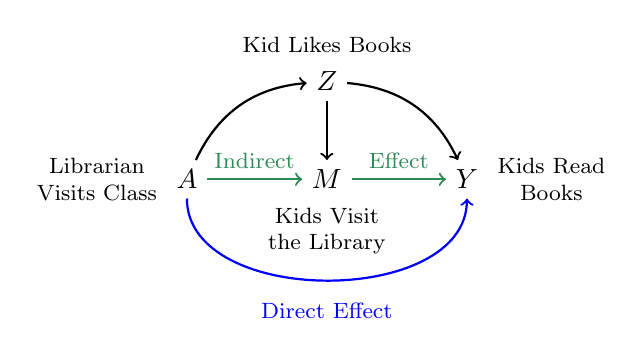
\begin{tikzpicture}[x = 1in, y = .7in, every node/.style = {anchor=center}]
\node (y) at (1.4,0) {$Y$};
\node[anchor = west, font = \footnotesize, align = center] at (y.east) {Kids Read\\Books};
\node (A) at (0,0) {$A$};
\node[anchor = east, font = \footnotesize, align = center] at (A.west) {Librarian\\Visits Class};
\node (M) at (.7,0) {$M$};
\node[anchor = north, font = \footnotesize, align = center] at (M.south) {Kids Visit\\the Library};
\draw[->, thick, seagreen] (A) -- node[midway, above, font = \footnotesize, seagreen] {Indirect} (M);
\draw[->, thick, seagreen] (M) -- node[midway, above, font = \footnotesize, seagreen] {Effect} (y);
\draw[->, thick, blue] (A) to[bend right = 90] node[midway, below, font = \footnotesize, outer sep = 5pt] {Direct Effect} (y);
\node (Z) at (.7,.7) {$Z$};
\node[anchor = south, font = \footnotesize, align = center] at (Z.north) {Kid Likes Books};
\draw[->, thick] (A) to[bend left] (Z);
\draw[->, thick] (Z) -- (M);
\draw[->, thick] (Z) to[bend left] (y);
\end{tikzpicture} \vskip .2in
\end{center}
Why? \pause For CDE:
$$\begin{aligned}
\E(Y^{10}) &= \E_{Z\mid A=1}\left(\E\left(Y\mid A = 1, M = 0, Z\right)\right)
\end{aligned}$$
\end{frame}

\begin{frame}[t]{Intermediate confounding: A threat to natural effects} \vskip .08in
\begin{center}
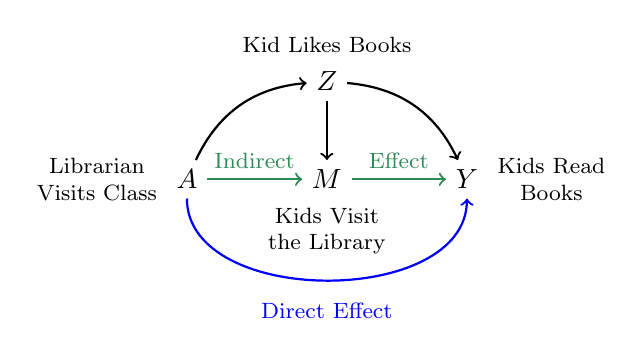
\begin{tikzpicture}[x = 1in, y = .7in, every node/.style = {anchor=center}]
\node (y) at (1.4,0) {$Y$};
\node[anchor = west, font = \footnotesize, align = center] at (y.east) {Kids Read\\Books};
\node (A) at (0,0) {$A$};
\node[anchor = east, font = \footnotesize, align = center] at (A.west) {Librarian\\Visits Class};
\node (M) at (.7,0) {$M$};
\node[anchor = north, font = \footnotesize, align = center] at (M.south) {Kids Visit\\the Library};
\draw[->, thick, seagreen] (A) -- node[midway, above, font = \footnotesize, seagreen] {Indirect} (M);
\draw[->, thick, seagreen] (M) -- node[midway, above, font = \footnotesize, seagreen] {Effect} (y);
\draw[->, thick, blue] (A) to[bend right = 90] node[midway, below, font = \footnotesize, outer sep = 5pt] {Direct Effect} (y);
\node (Z) at (.7,.7) {$Z$};
\node[anchor = south, font = \footnotesize, align = center] at (Z.north) {Kid Likes Books};
\draw[->, thick] (A) to[bend left] (Z);
\draw[->, thick] (Z) -- (M);
\draw[->, thick] (Z) to[bend left] (y);
\end{tikzpicture} \vskip .2in
\end{center}
Why? For NDE:
$$\begin{aligned}
\E(Y^{1M^0}) &= \E_{Z\mid A=1}\left(\E\left(Y\mid A = 1, M = M^0, Z\right)\right)
\end{aligned}$$
but we never have $M = M^0$ with $A = 1$, so that doesn't work
\end{frame}

\begin{frame}[t]{Intermediate confounding: A threat to natural effects} \vskip .08in
For NDE, this setting is nonparametrically identified
\begin{center}
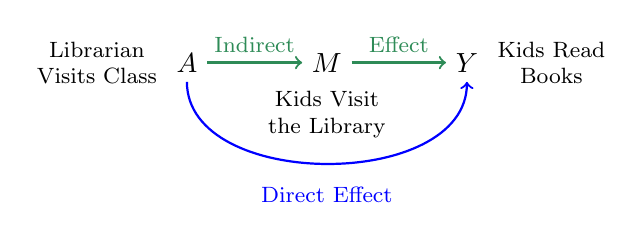
\begin{tikzpicture}[x = 1in, y = .7in, every node/.style = {anchor=center}]
\node (y) at (1.4,0) {$Y$};
\node[anchor = west, font = \footnotesize, align = center] at (y.east) {Kids Read\\Books};
\node (A) at (0,0) {$A$};
\node[anchor = east, font = \footnotesize, align = center] at (A.west) {Librarian\\Visits Class};
\node (M) at (.7,0) {$M$};
\node[anchor = north, font = \footnotesize, align = center] at (M.south) {Kids Visit\\the Library};
\draw[->, thick, seagreen] (A) -- node[midway, above, font = \footnotesize, seagreen] {Indirect} (M);
\draw[->, thick, seagreen] (M) -- node[midway, above, font = \footnotesize, seagreen] {Effect} (y);
\draw[->, thick, blue] (A) to[bend right = 90] node[midway, below, font = \footnotesize, outer sep = 5pt] {Direct Effect} (y);
%\node[white] (Z) at (.7,.7) {$Z$};
%\node[anchor = south, font = \footnotesize, align = center, white] at (Z.north) {Kid Likes Books};
%\draw[->, thick, white] (A) to[bend left] (Z);
%\draw[->, thick, white] (Z) -- (M);
%\draw[->, thick, white] (Z) to[bend left] (y);
\end{tikzpicture} \vskip .1in
\end{center} \pause
$$\begin{aligned}
\E(Y^{1M^0})  \pause
&= \E\left(Y\mid A = 1, M = M^0\right) \\ \pause
&= \P(M^0=1)\E\left(Y\mid A = 1, M = 1\right) \\ \pause
&\qquad + \P(M^0=0)\E\left(Y\mid A = 1, M = 0\right) \\
&= \P(M=1\mid A = 0)\E\left(Y\mid A = 1, M = 1\right) \\ \pause
&\qquad + \P(M=0\mid A = 0)\E\left(Y\mid A = 1, M = 0\right)  \pause
\end{aligned}$$
Identified because no potential outcomes remain!
\end{frame}

\begin{frame}{Estimation for NDE when sequential ignorability holds\footnote{Method implemented in the R package \texttt{mediation} and described on p.~773: Imai, K., Keele, L., Tingley, D., \& Yamamoto, T. (2011). \bref{https://doi.org/10.1017/S0003055411000414}{Unpacking the black box of causality: Learning about causal mechanisms from experimental and observational studies.} American Political Science Review, 105(4), 765-789.}}
\scalebox{.8}{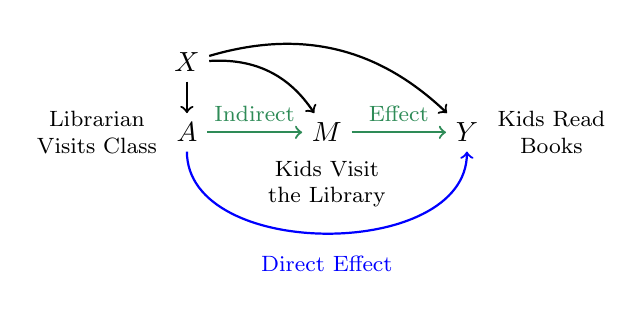
\begin{tikzpicture}[x = 1in, y = .7in, every node/.style = {anchor=center}]
\node (x) at (0,.5) {$X$};
\node (y) at (1.4,0) {$Y$};
\node[anchor = west, font = \footnotesize, align = center] at (y.east) {Kids Read\\Books};
\node (A) at (0,0) {$A$};
\node[anchor = east, font = \footnotesize, align = center] at (A.west) {Librarian\\Visits Class};
\node (M) at (.7,0) {$M$};
\node[anchor = north, font = \footnotesize, align = center] at (M.south) {Kids Visit\\the Library};
\draw[->, thick, seagreen] (A) -- node[midway, above, font = \footnotesize, seagreen] {Indirect} (M);
\draw[->, thick, seagreen] (M) -- node[midway, above, font = \footnotesize, seagreen] {Effect} (y);
\draw[->, thick, blue] (A) to[bend right = 90] node[midway, below, font = \footnotesize, outer sep = 5pt] {Direct Effect} (y);
\draw[->, thick] (x) -- (A);
\draw[->, thick] (x) to[bend left] (M);
\draw[->, thick] (x) to[bend left] (y);
\end{tikzpicture}} \pause \vskip .1in
\begin{enumerate}
\item Model $\E(M\mid X, A)$
\begin{itemize} \pause
\item Predict $M^a$ for all $a$
\end{itemize} \pause
\item Model $\E(Y\mid X, A,M)$
\begin{itemize} \pause
\item Predict $Y^{a',M^{a}}$ for any pair $a',a$
\end{itemize} \pause
\item Average over the sample.
\end{enumerate} \pause
Bootstrap for confidence intervals
\end{frame}

\begin{frame}{Summary: Mediation decomposes causal effects}
%\begin{itemize}
%\item
%\small
Controlled direct effects\hfill Example: $\E(Y^{10}-Y^{00})$
\begin{itemize}
\item Idea: Intervene to hold the mediator at a fixed value
\item \bgreen{\checkmark} Identified in a sequentially randomized experiment
\item \bgreen{\checkmark} Identifiable with observed intermediate confounding
\item \bred{X} Direct and indirect effects are not additively decomposable
\end{itemize} \vskip .1in
%\item 
Natural direct and indirect effects\hfill Example: $\E(Y^{1M^0}-Y^{0M^0})$
\begin{itemize}
\item Idea: Intervene to hold the mediator at the value in the absence of treatment
\item \bred{X} Not identified\footnote{Each use of ``identified'' refers to nonparametric identification. Parametric identification is sometimes possible when nonparametric identification is not.} in an experiment---$Y^{1M^0}$ is unobservable
\begin{itemize}
\item Crossover experiments can help with an extra assumption
\end{itemize}
\item \bred{X} Not identifiable with any intermediate confounding
\item \bgreen{\checkmark} Direct and indirect effects are additively decomposable
\end{itemize}
%\end{itemize}

\end{frame}

\goalsframe

\begin{frame}{Let me know what you are thinking}

\begin{huge} \bref{https://tinyurl.com/CausalQuestions}{tinyurl.com/CausalQuestions} \end{huge}
\vskip .7in

Office hours TTh 11am-12pm and at \bref{https://calendly.com/ianlundberg/office-hours}{calendly.com/ianlundberg/office-hours}\\Come say hi!

\end{frame}

\begin{frame}
SUPPLEMENTAL
\end{frame}
\begin{frame}{Natural direct and indirect effects in SWIGs}

Direct effect under mediator $M = M^1$\\
\begin{tikzpicture}[x = \textwidth]
\node[anchor = west] at (0,0) {
\scalebox{.8}{\begin{tikzpicture}[x = .8in]
\node (Amid) at (0,0) {$\mid$};
\node[anchor = east] (A) at (Amid.west) {$A$};
\node[anchor = west, blue] (a) at (Amid.east) {$1$};
\node (Mmid) at (1,0) {$\mid$};
\node[anchor = east] (M) at (Mmid.west) {$M$};
\node[anchor = west] (m) at (Mmid.east) {$M^1$};
\node (Mmid) at (2,0) {$Y$};
\node (Y) at (2,0) {$Y$};
\draw[->, thick] (a) -- (M);
\draw[->, thick] (m) -- (Y);
\draw[->, thick, line width = 2pt, blue] (a) to[bend left] (Y);
\end{tikzpicture}}
};
\node at (.5, 0) {$-$};
\node[anchor = west] at (.6,0) {
\scalebox{.8}{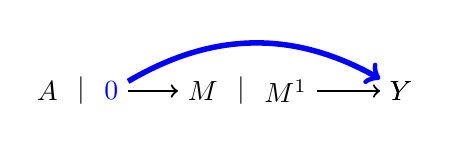
\begin{tikzpicture}[x = .8in]
\node (Amid) at (0,0) {$\mid$};
\node[anchor = east] (A) at (Amid.west) {$A$};
\node[anchor = west, blue] (a) at (Amid.east) {$0$};
\node (Mmid) at (1,0) {$\mid$};
\node[anchor = east] (M) at (Mmid.west) {$M$};
\node[anchor = west] (m) at (Mmid.east) {$M^1$};
\node (Mmid) at (2,0) {$Y$};
\node (Y) at (2,0) {$Y$};
\draw[->, thick] (a) -- (M);
\draw[->, thick] (m) -- (Y);
\draw[->, line width = 2pt, blue] (a) to[bend left] (Y);
\end{tikzpicture}}
};
\end{tikzpicture} \vskip .1in

Direct effect under mediator $M = M^0$\\
\begin{tikzpicture}[x = \textwidth]
\node[anchor = west] at (0,0) {
\scalebox{.8}{\begin{tikzpicture}[x = .8in]
\node (Amid) at (0,0) {$\mid$};
\node[anchor = east] (A) at (Amid.west) {$A$};
\node[anchor = west, blue] (a) at (Amid.east) {$1$};
\node (Mmid) at (1,0) {$\mid$};
\node[anchor = east] (M) at (Mmid.west) {$M$};
\node[anchor = west] (m) at (Mmid.east) {$M^0$};
\node (Mmid) at (2,0) {$Y$};
\node (Y) at (2,0) {$Y$};
\draw[->, thick] (a) -- (M);
\draw[->, thick] (m) -- (Y);
\draw[->, thick, line width = 2pt, blue] (a) to[bend left] (Y);
\end{tikzpicture}}
};
\node at (.5, 0) {$-$};
\node[anchor = west] at (.6,0) {
\scalebox{.8}{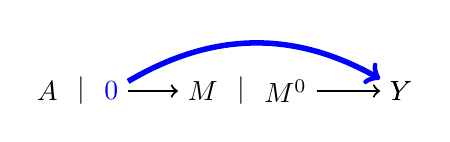
\begin{tikzpicture}[x = .8in]
\node (Amid) at (0,0) {$\mid$};
\node[anchor = east] (A) at (Amid.west) {$A$};
\node[anchor = west, blue] (a) at (Amid.east) {$0$};
\node (Mmid) at (1,0) {$\mid$};
\node[anchor = east] (M) at (Mmid.west) {$M$};
\node[anchor = west] (m) at (Mmid.east) {$M^0$};
\node (Mmid) at (2,0) {$Y$};
\node (Y) at (2,0) {$Y$};
\draw[->, thick] (a) -- (M);
\draw[->, thick] (m) -- (Y);
\draw[->, thick, line width = 2pt, blue] (a) to[bend left] (Y);
\end{tikzpicture}}
};
\end{tikzpicture} \vskip .1in

Indirect effect under treatment $A = 1$\\
\begin{tikzpicture}[x = \textwidth]
\node[anchor = west] at (0,0) {
\scalebox{.8}{\begin{tikzpicture}[x = .8in]
\node (Amid) at (0,0) {$\mid$};
\node[anchor = east] (A) at (Amid.west) {$A$};
\node[anchor = west] (a) at (Amid.east) {$1$};
\node (Mmid) at (1,0) {$\mid$};
\node[anchor = east] (M) at (Mmid.west) {$M$};
\node[anchor = west, blue] (m) at (Mmid.east) {$M^1$};
\node (Mmid) at (2,0) {$Y$};
\node (Y) at (2,0) {$Y$};
\draw[->, thick] (a) -- (M);
\draw[->, line width = 2pt, blue] (m) -- (Y);
\draw[->, thick] (a) to[bend left] (Y);
\end{tikzpicture}}
};
\node at (.5, 0) {$-$};
\node[anchor = west] at (.6,0) {
\scalebox{.8}{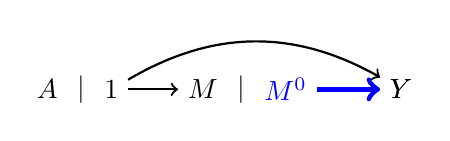
\begin{tikzpicture}[x = .8in]
\node (Amid) at (0,0) {$\mid$};
\node[anchor = east] (A) at (Amid.west) {$A$};
\node[anchor = west] (a) at (Amid.east) {$1$};
\node (Mmid) at (1,0) {$\mid$};
\node[anchor = east] (M) at (Mmid.west) {$M$};
\node[anchor = west, blue] (m) at (Mmid.east) {$M^0$};
\node (Mmid) at (2,0) {$Y$};
\node (Y) at (2,0) {$Y$};
\draw[->, thick] (a) -- (M);
\draw[->, line width = 2pt, blue] (m) -- (Y);
\draw[->, thick] (a) to[bend left] (Y);
\end{tikzpicture}}
};
\end{tikzpicture} \vskip .1in

Indirect effect under treatment $A = 0$\\
\begin{tikzpicture}[x = \textwidth]
\node[anchor = west] at (0,0) {
\scalebox{.8}{\begin{tikzpicture}[x = .8in]
\node (Amid) at (0,0) {$\mid$};
\node[anchor = east] (A) at (Amid.west) {$A$};
\node[anchor = west] (a) at (Amid.east) {$0$};
\node (Mmid) at (1,0) {$\mid$};
\node[anchor = east] (M) at (Mmid.west) {$M$};
\node[anchor = west, blue] (m) at (Mmid.east) {$M^1$};
\node (Mmid) at (2,0) {$Y$};
\node (Y) at (2,0) {$Y$};
\draw[->, thick] (a) -- (M);
\draw[->, line width = 2pt, blue] (m) -- (Y);
\draw[->, thick] (a) to[bend left] (Y);
\end{tikzpicture}}
};
\node at (.5, 0) {$-$};
\node[anchor = west] at (.6,0) {
\scalebox{.8}{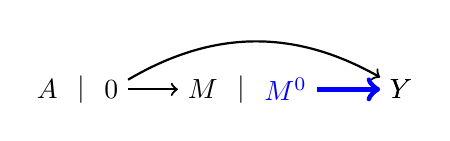
\begin{tikzpicture}[x = .8in]
\node (Amid) at (0,0) {$\mid$};
\node[anchor = east] (A) at (Amid.west) {$A$};
\node[anchor = west] (a) at (Amid.east) {$0$};
\node (Mmid) at (1,0) {$\mid$};
\node[anchor = east] (M) at (Mmid.west) {$M$};
\node[anchor = west, blue] (m) at (Mmid.east) {$M^0$};
\node (Mmid) at (2,0) {$Y$};
\node (Y) at (2,0) {$Y$};
\draw[->, thick] (a) -- (M);
\draw[->, line width = 2pt, blue] (m) -- (Y);
\draw[->, thick] (a) to[bend left] (Y);
\end{tikzpicture}}
};
\end{tikzpicture}

\end{frame}

\end{document}